\section{Experimentos Preliminares}

\subsection{Conjunto de dados UCI}
\begin{frame}{Repositório da Universidade da Califórnia em Irvine}
  \begin{itemize}
  
  \item Contém 245.057 amostras obtidas de imagens do PAL e FERET \citep{pal-texas:04, feret:96}
  
  \item 194.198 são de pixels não pele e 50.859 de pixels de pele
  
  \item Compostas por 3 atributos $x = [x_1, x_2, x_3]$, $x \in \mathbb{R}^{3}$, que representam os canais do modelo de cores RGB
  
  \item Uma quarta coluna determina a classe a qual a amostra $x$ pertence, denotada por $y$, sendo $y \in Y$ e $Y = \{+1, -1\}$
  \end{itemize}
\end{frame}

%------------------------------------------------------
\begin{frame}{Amostras do conjunto de dados}
\begin{table}[!htpb]
\centering
\begin{small}
\begin{tabular}{|c|c|c|c|} \hline
\thb{B} & \thb{G} & \thb{R}  & \thb{Classe}  \\ \hline
74	    & 85      & 123	     & 1     \\
207	    & 215     & 255      & 1     \\
74      & 82      & 122	     & 1     \\
202     & 211     & 255      & 1     \\
54      & 72      & 125      & 1     \\
\ldots  &\ldots   & \dots    &\ldots \\
166     & 164     & 116      & -1    \\
148     & 150     & 91       & -1    \\
29      & 26      & 5        & -1    \\
167     & 166	  & 115	     & -1    \\
180	    & 177	  & 133	     & -1    \\ \hline
\end{tabular}
\end{small}
\end{table}
\end{frame}

%------------------------------------------------------
\begin{frame}{Visão 3-dimensional dos canais RGB}
\begin{figure}[h]
    \centering
    \begin{minipage}{0.45\textwidth}
        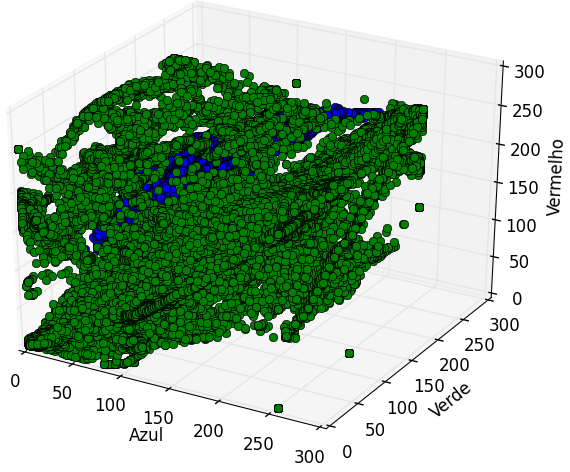
\includegraphics[width=\textwidth]{uci_skinns_plot}
    \end{minipage}
    ~ % space
    \begin{minipage}{0.45\textwidth}
        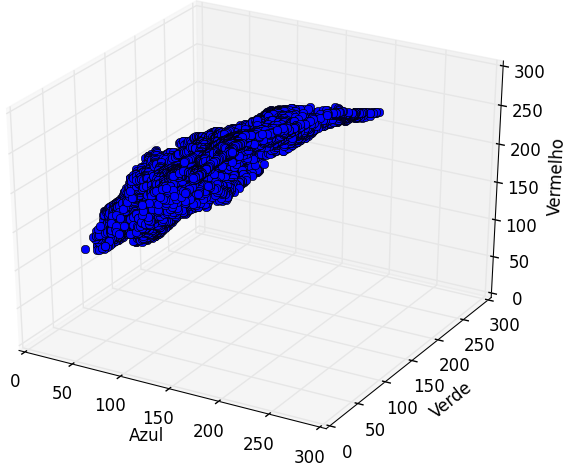
\includegraphics[width=\textwidth]{uci_skin_plot}
    \end{minipage}
    \label{fig:dataset_uci}
\end{figure}
\end{frame}

%------------------------------------------------------
\subsection{Conjunto de dados SFA}
\begin{frame}{Banco de imagens de faces do FERET e AR}
  \begin{itemize}
      \item 876 imagens de faces obtidas do FERET, criado por \citet{feret:96} e 242 do AR, proposto por \citet{ar-face-database:98}
      
      \item As imagens do AR têm fundo branco e pequenas variações de cor da pele e, portanto, o ambiente é mais controlado
      
      \item Três amostras de pele e cinco não pele foram geradas aleatoriamente considerando a máscara \emph{ground truth} de cada imagem
  \end{itemize}
\end{frame}

%------------------------------------------------------
\begin{frame}{Exemplos de imagens do banco de faces}
\begin{figure}[h]
    \centering
    \begin{subfigure}[t]{0.17\textwidth}
        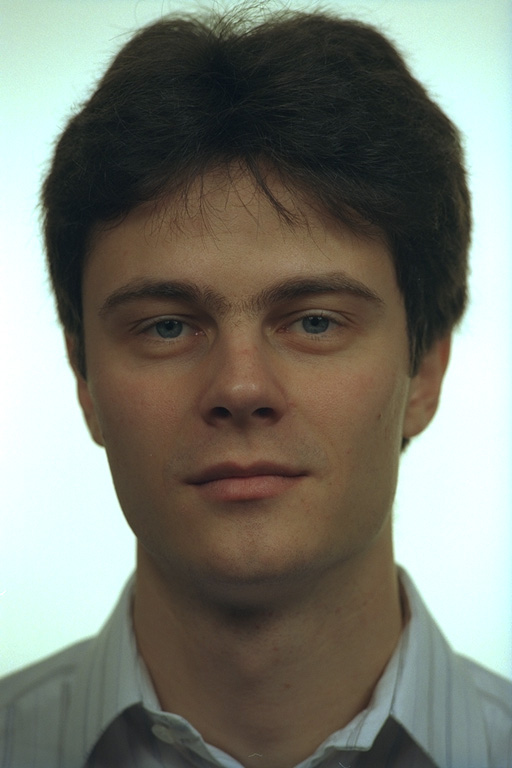
\includegraphics[width=\textwidth]{sfa_img_1}\\
        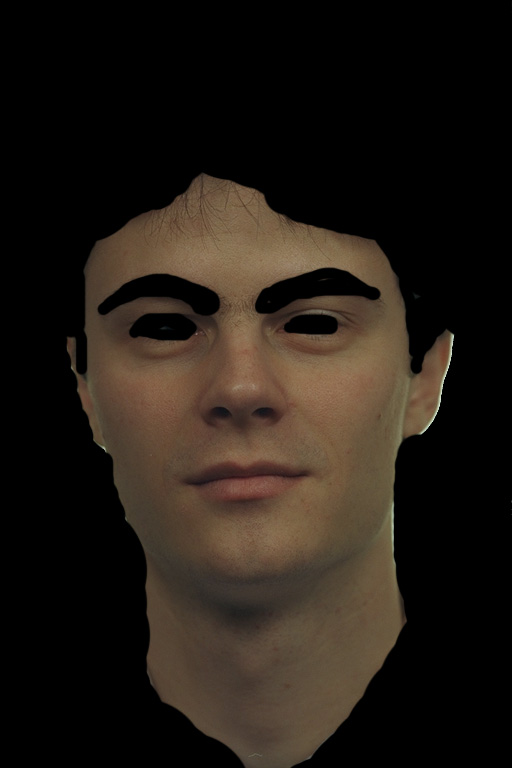
\includegraphics[width=\textwidth]{sfa_img_1_gt}
    \end{subfigure}
    ~
    \begin{subfigure}[t]{0.17\textwidth}
        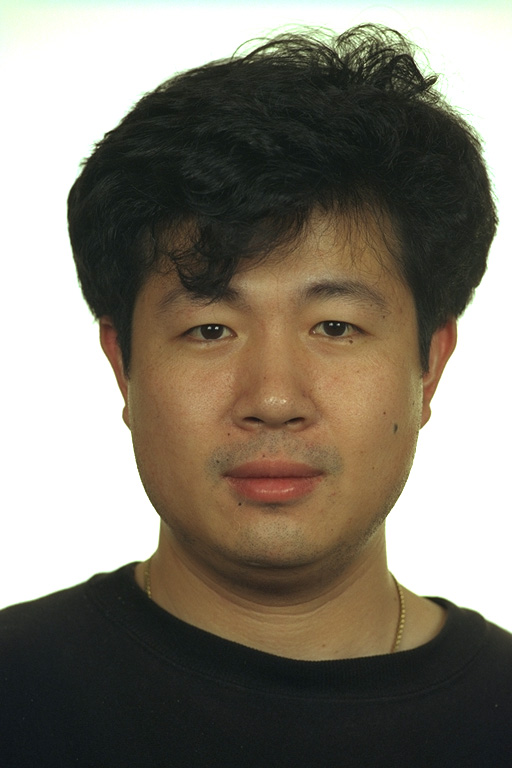
\includegraphics[width=\textwidth]{sfa_img_14}\\
        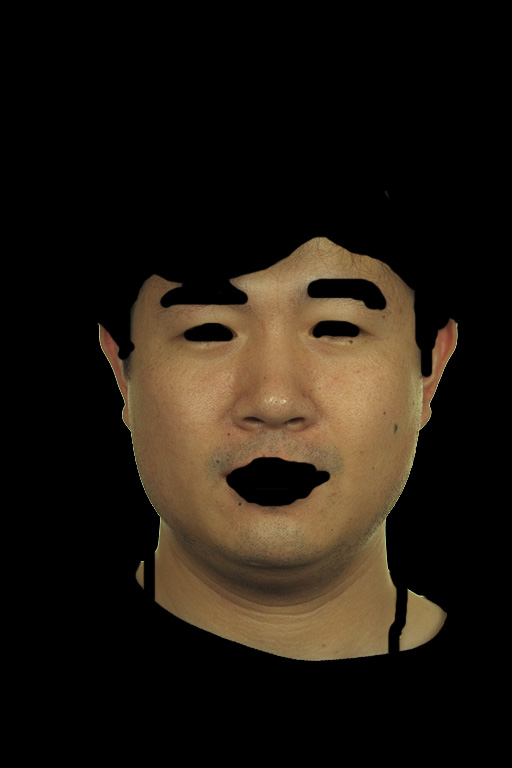
\includegraphics[width=\textwidth]{sfa_img_14_gt}
    \end{subfigure}
    ~
    \begin{subfigure}[t]{0.17\textwidth}
        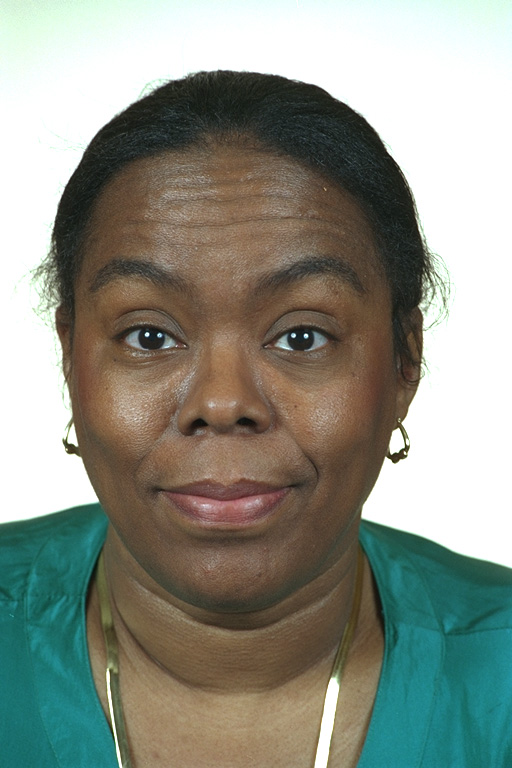
\includegraphics[width=\textwidth]{sfa_img_586}\\
        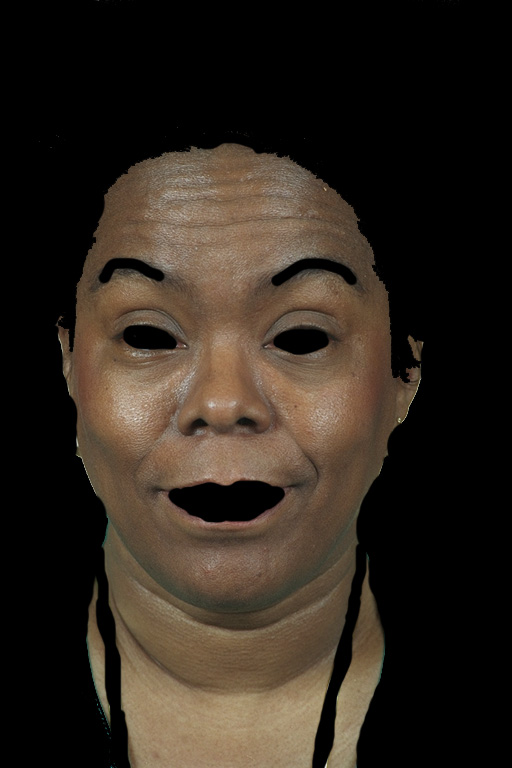
\includegraphics[width=\textwidth]{sfa_img_586_gt}
    \end{subfigure}
    ~ % space
    \begin{subfigure}[t]{0.17\textwidth}
        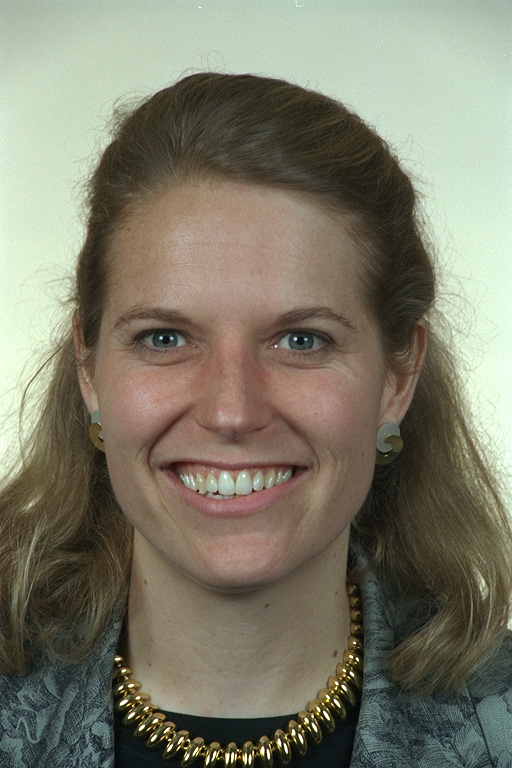
\includegraphics[width=\textwidth]{sfa_img_726}\\
        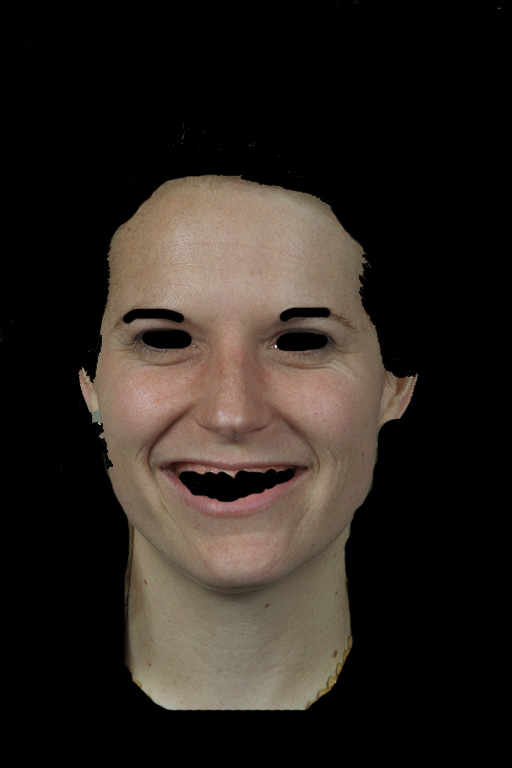
\includegraphics[width=\textwidth]{sfa_img_726_gt}
    \end{subfigure}
\end{figure}
\end{frame}

%------------------------------------------------------
\begin{frame}{Estrutura das janelas}
  \begin{itemize}
      \item Cada amostra é uma janela de tamanho $n\times n$, sendo $n$ ímpar, que varia de $1 \times 1$ até $35 \times 35$
      
      \item O conjunto de dados foi gerado com janela $9 \times 9$, totalizando 724.464 amostras, sendo 271.674 de pele e 452.790 não pele
  \end{itemize}

  \begin{figure}
    \centering
    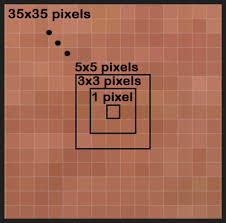
\includegraphics[width=.3\textwidth]{sfa-janelas}
  \end{figure}
\end{frame}

%------------------------------------------------------
\begin{frame}{Visão 3-dimensional dos canais RGB}
\begin{figure}[h]
    \centering
    \begin{minipage}{0.45\textwidth}
        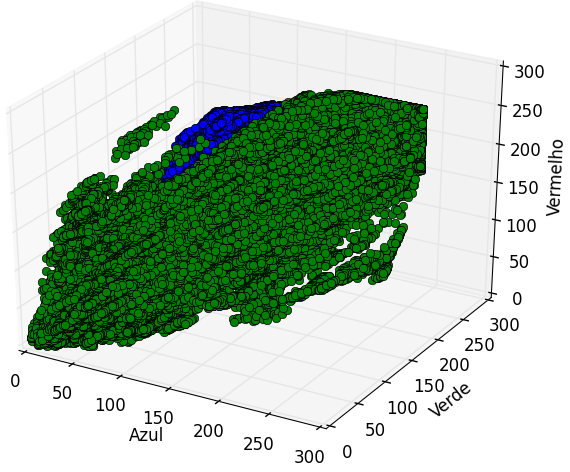
\includegraphics[width=\textwidth]{sfa_skinns_plot}
    \end{minipage}
    ~ % space
    \begin{minipage}{0.45\textwidth}
        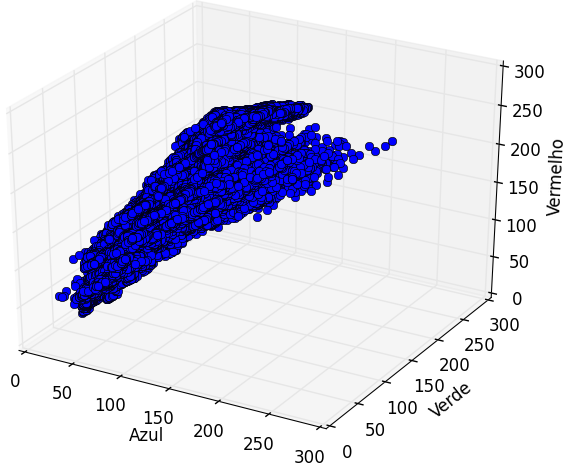
\includegraphics[width=\textwidth]{sfa_skin_plot}
    \end{minipage}
\end{figure}
\end{frame}

%------------------------------------------------------
\subsection{Primeiro experimento}
\begin{frame}{Primeiro experimento}
  \begin{itemize}
      \item Realizado com $k$-NN e SVM no espaço de cores RGB
      \item Estratégia de validação cruzada \emph{10-fold} em ambos
      \item Os parâmetros ótimos foram:
      \begin{itemize}
          \item \textbf{\emph{k}-NN:} \emph{n\_neighbors}=3, \emph{weights=uniform} no UCI e \emph{n\_neighbors}=15, \emph{weights=uniform} no SFA
          \item \textbf{SVM:} \emph{kernel=rbf}, C=100 e \emph{gamma}=1e-3 em ambos UCI e SFA
      \end{itemize}
  \end{itemize}
\end{frame}

%------------------------------------------------------
\begin{frame}{Tabela de busca}
\begin{table}[!htpb]
\centering
\begin{small}
\setlength{\tabcolsep}{8pt}

\begin{tabular}{|c|c|c|c|c|c|c|c|c|c|}\hline
 \thbi{kernel} & \multicolumn{4}{c|}{\thbi{C}} & \multicolumn{3}{c|}{\thbi{gamma}} & \multicolumn{2}{c|}{\thbi{degree}}\\ \cline{1-10}
rbf    & 1 & 10 & 100 & 1000 & 1e-3 & 1e-4 & 1e-5 &   &   \\ \hline
poly   & 1 & 10 & 100 & 1000 &      & 1e-4 & 1e-5 & 3 & 4 \\ \hline
linear & 1 & 10 & 100 & 1000 &      &      &      &   &   \\ \hline

\end{tabular}
\end{small}
\caption{Tabela de busca dos parâmetros do estimador ótimo na SVM.}
\end{table}

\begin{table}[!htpb]
\centering
\begin{small}
\setlength{\tabcolsep}{3.6pt}

\begin{tabular}{|c|c|c|c|c|c|c|c|c|c|c|c|c|}\hline
 \multicolumn{10}{|c|}{\thbi{n\_neighbors}} & \multicolumn{2}{c|}{\thbi{weights}} & \multicolumn{1}{c|}{\thbi{algorithm}}\\ \cline{1-13}
3 & 5 & 9 & 15 & 25 & 50 & 100 & 200 & 400 & 800 & distance & uniform & auto \\ \hline

\end{tabular} 
\end{small}
\caption{Tabela de busca dos parâmetros do estimador ótimo no k-NN.}
\end{table}
\end{frame}

%------------------------------------------------------
\begin{frame}{Resultados}
O treinamento foi executado com 10 tarefas em paralelo em ambos os classificadores e 30\% dos dados, aleatoriamente, foram separados para teste.
\begin{table}[!htpb]
\centering
\begin{small}
\setlength{\tabcolsep}{4pt}

\begin{tabular}{|c|c|c|c|c|c|}\hline
 \thb{Dados} & \thb{Classificador} & \thb{Modelo de cores} & \thbi{Precision} & \thbi{Recall} & \thbi{F1-score} \\ \hline
 \multirow{2}{*}{UCI} & $k$-NN & RGB & 0,9995 & 0,9995 & 0,9995 \\ \cline{2-6}
                      & SVM    & RGB & 0,9995 & 0,9995 & 0,9995 \\ \hline
 \multirow{2}{*}{SFA} & $k$-NN & RGB & 0,9672 & 0,9669 & 0,9670 \\ \cline{2-6}
                      & SVM    & RGB & 0,9643 & 0,9628 & 0,9638 \\ \hline

\end{tabular}
\end{small}
\end{table}
\end{frame}

%------------------------------------------------------
\subsection{Segundo experimento}
\begin{frame}{Segundo experimento}
    \begin{itemize}
        \item Realizado com $k$-NN e SVM usando o conjunto de dados SFA nos espaços de cores RGB, HSV, Lab e YCbCr
        \item O componente de luminância foi ignorado para que um teste somente com os componentes de crominância fosse realizado
        \item Estratégia escolhida de validação cruzada \emph{10-fold}
        \item Os parâmetros ótimos obtidos no primeiro experimento foram fixados aqui
        \item Treinamento com 10 tarefas em paralelo, 30\% dos dados, aleatoriamente, foram separados para teste
    \end{itemize}
\end{frame}

%------------------------------------------------------
\begin{frame}{Resultados}
\begin{table}[!htpb]
\centering
\begin{small}
\setlength{\tabcolsep}{4pt}

\begin{tabular}{|c|c|c|c|c|}\hline
 Modelo de cores & Classificador & \emph{Precision} & \emph{Recall} & \emph{F1-score} \\ \hline
 \multirow{2}{*}{RGB}   & $k$-NN  & 0,9672 & 0,9669 & 0,9670 \\ \cline{2-5}
                        & SVM     & 0,9643 & 0,9628 & 0,9638 \\ \hline
 \multirow{2}{*}{HSV}   & $k$-NN  & 0,9676 & 0,9673 & 0,9674 \\ \cline{2-5}
                        & \alert{SVM}     & \alert{0,9718} & \alert{0,9677} & \alert{0,9679} \\ \hline
 \multirow{2}{*}{HS}    & $k$-NN  & 0,9215 & 0,9194 & 0,9199 \\ \cline{2-5}
                        & SVM     & 0,9305 & 0,9302 & 0,9302 \\ \hline
 \multirow{2}{*}{Lab}   & $k$-NN  & 0,9671 & 0,9660 & 0,9670 \\ \cline{2-5}
                        & SVM     & 0,9675 & 0,9665 & 0,9672 \\ \hline
 \multirow{2}{*}{ab}    & $k$-NN  & 0,9444 & 0,9439 & 0,9440 \\ \cline{2-5}
                        & SVM     & 0,9451 & 0,9447 & 0,9446 \\ \hline
 \multirow{2}{*}{YCbCr} & \alert{$k$-NN}  & \alert{0,9679} & \alert{0,9677} & \alert{0,9677} \\ \cline{2-5}
                        & SVM     & 0,9635 & 0,9633 & 0,9632 \\ \hline
 \multirow{2}{*}{CbCr}  & \alert{$k$-NN}  & \alert{0,9487} & \alert{0,9482} & \alert{0,9483} \\ \cline{2-5}
                        & \alert{SVM}     & \alert{0,9496} & \alert{0,9492} & \alert{0,9493} \\ \hline

\end{tabular}
\end{small}
\end{table}
\end{frame}

%------------------------------------------------------
\subsection{Terceiro experimento}
\begin{frame}{Terceiro experimento}
    \begin{itemize}
        \item Realizado com árvore de decisão \emph{fuzzy} proposta por \citet{cintra:13} usando o conjunto de dados SFA nos espaços de cores RGB, HSV, Lab e YCbCr
        \item Os parâmetros do \emph{FuzzyDT} podem ser customizados para determinar a poda da árvore e o método de estimativa do número de conjuntos \emph{fuzzy} por atributo
        \item Desenvolvido um algoritmo de tabela de busca para encontrar os parâmetros ótimos
    \end{itemize}
\end{frame}

%------------------------------------------------------
\begin{frame}{Tabela de busca}
\begin{table}[!htpb]
\centering
\begin{small}
\setlength{\tabcolsep}{5pt}

\begin{tabular}{|c|c|c|c|c|c|c|c|c|c|}\hline
 \thb{Dados} & \multicolumn{4}{c|}{\thb{Nível de confiança}} & \multicolumn{4}{c|}{\thb{Método}} & \thb{\texttt{\#} conj. \emph{fuzzy}}\\ \cline{1-10}
RGB   & 10 & 15 & 20 & 25 & infogain & wm & rf & fixed & 2-9 \\ \hline
HSV   & 10 & 15 & 20 & 25 & infogain & wm & rf & fixed & 2-9 \\ \hline
Lab   & 10 & 15 & 20 & 25 & infogain & wm & rf & fixed & 2-9 \\ \hline
YCbCr & 10 & 15 & 20 & 25 & infogain & wm & rf & fixed & 2-9 \\ \hline

\end{tabular}
\end{small}
\end{table}
\end{frame}

%------------------------------------------------------
\begin{frame}{Resultados}
\begin{table}[!htpb]
\centering
\begin{small}
\setlength{\tabcolsep}{6pt}

\begin{tabular}{|c|c|c|c|}\hline
 \thb{Modelo de cores} & \thb{Taxa de erro} & \thb{Método} & \thb{\texttt{\#} conjuntos \emph{fuzzy}} \\ \hline
 RGB   & 3,00 & fixed & 4 \\ \hline
 HSV   & 3,23 & fixed & 3 \\ \hline
 Lab   & 2,84 & fixed & 6 \\ \hline
 YCbCr & 2,72 & fixed & 8 \\ \hline

\end{tabular}
\end{small}
\end{table}
\end{frame}